\documentclass{article}

\usepackage{amsmath, amsthm, amssymb, amsfonts}
\usepackage{thmtools}
\usepackage{graphicx}
\usepackage{setspace}
\usepackage{geometry}
\usepackage{float}
\usepackage{hyperref}
\usepackage[utf8]{inputenc}
\usepackage[english]{babel}
\usepackage{framed}
\usepackage[dvipsnames]{xcolor}
\usepackage{tcolorbox}

%Define the listing package
\usepackage{listings} %code highlighter
\usepackage{color} %use color
\definecolor{mygreen}{rgb}{0,0.6,0}
\definecolor{mygray}{rgb}{0.5,0.5,0.5}
\definecolor{mymauve}{rgb}{0.58,0,0.82}
 
%Customize a bit the look
\lstset{ %
backgroundcolor=\color{white}, % choose the background color; you must add \usepackage{color} or \usepackage{xcolor}
basicstyle=\footnotesize, % the size of the fonts that are used for the code
breakatwhitespace=false, % sets if automatic breaks should only happen at whitespace
breaklines=true, % sets automatic line breaking
captionpos=b, % sets the caption-position to bottom
commentstyle=\color{mygreen}, % comment style
deletekeywords={...}, % if you want to delete keywords from the given language
escapeinside={\%*}{*)}, % if you want to add LaTeX within your code
extendedchars=true, % lets you use non-ASCII characters; for 8-bits encodings only, does not work with UTF-8
frame=single, % adds a frame around the code
keepspaces=true, % keeps spaces in text, useful for keeping indentation of code (possibly needs columns=flexible)
keywordstyle=\color{blue}, % keyword style
% language=Octave, % the language of the code
morekeywords={*,...}, % if you want to add more keywords to the set
numbers=left, % where to put the line-numbers; possible values are (none, left, right)
numbersep=5pt, % how far the line-numbers are from the code
numberstyle=\tiny\color{mygray}, % the style that is used for the line-numbers
rulecolor=\color{black}, % if not set, the frame-color may be changed on line-breaks within not-black text (e.g. comments (green here))
showspaces=false, % show spaces everywhere adding particular underscores; it overrides 'showstringspaces'
showstringspaces=false, % underline spaces within strings only
showtabs=false, % show tabs within strings adding particular underscores
stepnumber=1, % the step between two line-numbers. If it's 1, each line will be numbered
stringstyle=\color{mymauve}, % string literal style
tabsize=2, % sets default tabsize to 2 spaces
title=\lstname % show the filename of files included with \lstinputlisting; also try caption instead of title
}
%END of listing package%
 
\definecolor{darkgray}{rgb}{.4,.4,.4}
\definecolor{purple}{rgb}{0.65, 0.12, 0.82}
 
%define Javascript language
\lstdefinelanguage{JavaScript}{
keywords={typeof, new, true, false, catch, function, return, null, catch, switch, var, if, in, while, do, else, case, break},
keywordstyle=\color{blue}\bfseries,
ndkeywords={class, export, boolean, throw, implements, import, this},
ndkeywordstyle=\color{darkgray}\bfseries,
identifierstyle=\color{black},
sensitive=false,
comment=[l]{//},
morecomment=[s]{/*}{*/},
commentstyle=\color{purple}\ttfamily,
stringstyle=\color{red}\ttfamily,
morestring=[b]',
morestring=[b]"
}
 
\lstset{
language=JavaScript,
extendedchars=true,
basicstyle=\footnotesize\ttfamily,
showstringspaces=false,
showspaces=false,
numbers=left,
numberstyle=\footnotesize,
numbersep=9pt,
tabsize=2,
breaklines=true,
showtabs=false,
captionpos=b
}

\lstdefinelanguage{C}{
keywords={typeof, new, true, false, catch, function, return, null, catch, switch, var, if, in, while, do, else, case, break},
keywordstyle=\color{blue}\bfseries,
ndkeywords={class, export, boolean, throw, implements, import, this},
ndkeywordstyle=\color{darkgray}\bfseries,
identifierstyle=\color{black},
sensitive=false,
comment=[l]{//},
morecomment=[s]{/*}{*/},
commentstyle=\color{purple}\ttfamily,
stringstyle=\color{red}\ttfamily,
morestring=[b]',
morestring=[b]"
}

\colorlet{LightGray}{White!90!Periwinkle}
\colorlet{LightOrange}{Orange!15}
\colorlet{LightGreen}{Green!15}

\newcommand{\HRule}[1]{\rule{\linewidth}{#1}}

\NewEnviron{NORMAL}{% 
    \scalebox{2}{$\BODY$} 
} 

\declaretheoremstyle[name=Theorem,]{thmsty}
\declaretheorem[style=thmsty,numberwithin=section]{theorem}
\tcolorboxenvironment{theorem}{colback=LightGray}

\declaretheoremstyle[name=Proposition,]{prosty}
\declaretheorem[style=prosty,numberlike=theorem]{proposition}
\tcolorboxenvironment{proposition}{colback=LightOrange}

\declaretheoremstyle[name=Principle,]{prcpsty}
\declaretheorem[style=prcpsty,numberlike=theorem]{principle}
\tcolorboxenvironment{principle}{colback=LightGreen}

\setstretch{1.2}
\geometry{
    textheight=9in,
    textwidth=5.5in,
    top=1in,
    headheight=12pt,
    headsep=25pt,
    footskip=30pt
}

% ------------------------------------------------------------------------------

\begin{document}

% ------------------------------------------------------------------------------
% Cover Page and ToC
% ------------------------------------------------------------------------------

\title{ \normalsize \textsc{}
		\\ [2.0cm]
		\HRule{1.5pt} \\
		\LARGE \textbf{\uppercase{Base di Dati}
		\HRule{2.0pt} \\ [0.6cm] \LARGE{Corso A} \vspace*{10\baselineskip}}
		}
        
\date{\text{Ultima Compilazione - }\today}
\author{\textbf{Autore} \\ 
		Giuseppe Acocella \\
		2025/26\\
        \url{https://github.com/Peenguino}}

\maketitle
\newpage

\tableofcontents

\newpage

\section{Introduzione}

I database sono insiemi di dati omogenei gestiti in collezioni. Alla base di questo definiamo tabelle, i cui campi possono fare riferimento ad altre tabelle
del database. Il topic di studio del corso è quello dei \textbf{database}, ma in questa introduzione definiamo un confronto con i \textbf{Data Warehouse}, per evidenziarne le \textbf{differenze}, anche
non essendo parte del programma del corso. 

\subsection{OLTP vs OLAP}

Mettiamo a confronto i due tipi di \textbf{ambiti applicativi}:

\begin{enumerate}
    \item \textbf{OLTP - Database (transazionale)}:
    \begin{enumerate}
        \item Utilizzo comune.
        \item Molti users.
        \item Dati analitici e relazionali.
        \item Relazioni statiche.
        \item Una query altera solitamente pochi record della tabella.
        \item Mirato all'utilizzo da parte delle applicazioni.
        \item Aggiornamenti frequenti.
        \item Visione dei dati correnti.
        \item Pensato per le transazioni.
    \end{enumerate}
    \item \textbf{OLAP - Data Warehouse (analitico)}:
    \begin{enumerate}
        \item Pochi utenti esperti.
        \item Dati multidimensionali.
        \item Relazioni dinamiche.
        \item Una query altera molti record della tabella.
        \item Mirato ai soggetti.
        \item Aggiornamenti rari ma massivi.
        \item Visione dei dati storica.
        \item Pensato per l'analisi di trend.
    \end{enumerate}
\end{enumerate}

Per questa motivazione, se dei dati presenti in un database, dovessero servire per un analisi di trend andrebbe effettuata un operazione abbastanza complessa di
estrazione e preparazione per l'immagazzinamento nel Data Warehouse. Entrambi (DB e DW) seguono una politica \textbf{schema first}, ossia viene prima definito uno schema
(insieme di campi) su cui verrà basata la successiva popolazione della collezione di informazioni.

\paragraph{Big Data} Un esempio di collezione di dati che \textbf{non segue} una politica \textbf{schema first}, basandosi infatti sulle proprietà di volume, varietà e velocità
non possono mantenere la rigidità impostata da uno schema. Solitamente sono quindi associati a sistemi NoSQL o approcci Data Lake.

\newpage

\subsection{Data Base Management Systems - DBMS}

Un DBMS (sistema per basi di dati) è un sistema centralizzato o distribuito che offre opportuni linguaggi per:

\begin{enumerate}
    \item Definire lo \textbf{schema} di una DB.
    \item Scegliere le \textbf{strutture dati} a \textbf{supporto} della DB.
    \item \textbf{Memorizzare} dati seguendo i vincoli definiti dai schemi del DB.
    \item Recuperare e modificare dati del DB tramite interrogazioni (\textbf{query}).
\end{enumerate}

Solitamente si pone tra i programmi applicativi e l'effettivo database per permettere l'interazione vincolata tra i due.

\paragraph{Dati gestiti dai DBMS}

Solitamente in un DB sono contenuti:

\begin{enumerate}
    \item \textbf{Metadati}: Descrivono permessi, applicazioni, parametri quantitativi sui dati effettivi. Seguono uno schema definito dal DBMS stesso.
    \item \textbf{Dati}: Rappresentazioni di fatti conformi alle definizioni degli schemi del DB.
    \begin{enumerate}
        \item Sono organizzati in \textbf{insiemi} strutturati ed \textbf{omogenei}, tra i quali sono definite delle \textbf{relazioni}.
        \item Sono accessibili tramite \textbf{transazioni}, operazioni atomiche che non hanno \textbf{mai effetti parziali}.
        \item Sono protetti da accessi non autorizzati e preservati da possibili malfunzionamenti.
        \item Sono utilizzabili in maniera concorrente da più utenti.
    \end{enumerate}
\end{enumerate}

\paragraph{DBMS a Modello Relazionale} Il modello relazionale è il più comune tra i DBMS commerciali e si basa sull'astrazione della \textbf{relazione}, ossia la \textbf{tabella}
vista come un insieme di record con campi ben definiti. Questo ci permette di poter creare tabelle ed interrogarle con un linguaggio ad alto livello.

\paragraph{Funzionalità dei DBMS} Elenchiamo quindi le proprietà garantite da un DBMS:

\begin{enumerate}
    \item Linguaggio per la definizione di un DB.
    \item Linguaggio per l'uso dei dati nel DB.
    \item Meccanismi di controllo del DB.
    \item Strumenti per la gestione admin del DB.
    \item Strumenti per lo sviluppo delle app che richiedono dati dal DB.
\end{enumerate}

\newpage

\subsubsection{Livelli di Vista Dati dei DBMS}

Per garantire le proprietà di \textbf{indipendenza fisica} e \textbf{logica} dei dati è stato proposto l'approccio di tre livelli di descrizione dei dati.

\begin{enumerate}
    \item \textbf{Indipendenza Fisica}: Le applicazioni che utilizzano il DB \textbf{non} devono essere modificati in seguito a modifiche dell'organizzazione fisica
    dei dati nel DB.
    \item \textbf{Indipendenza Logica}: Le applicazioni che utilizzano il DB \textbf{non} devono essere modificati in seguito a modifiche dello schema logico del DB.
\end{enumerate}

Gli effettivi livelli di vista sono invece:

\begin{enumerate}
    \item \textbf{Livello Fisico}: Gestione effettiva dell'immagazzinamento dei dati nel DB, ad esempio in questo livello si scelgono le strutture dati e gli algoritmi
    utilizzati dal DBMS per navigare tra i dati.
    \item \textbf{Livello Logico}: Descrizione della struttura degli insiemi di dati e delle relazioni tra di loro, astraendo completamente dalla loro gestione fisica.
    \item \textbf{Livello Vista Logica}: Sottoinsieme del livello logico esposto alle applicazioni esterne.
\end{enumerate}

\subsubsection{Meccanismi di Controllo Dati e Transazioni dei DBMS}

I DBMS cercano di garantire queste proprietà sui dati immagazzinati in un DB:

\begin{enumerate}
    \item \textbf{Integrità}: Mantenimento delle proprietà definite dallo schema.
    \item \textbf{Sicurezza}: Protezione dei dati da usi non autorizzati.
    \item \textbf{Affidabilità}: Protezione in caso di malfunzionamenti hardware/software.
\end{enumerate}

\paragraph{Transazioni - Operazioni Atomiche} Una transazione è una sequenza di azioni di lettura e scrittura in memoria permanente e di elaborazioni di dati in memoria
temporanea secondo queste proprietà:

\begin{enumerate}
    \item \textbf{Atomicità}: Le transazioni terminate prematuramente sono trattate come se non fossero mai iniziate. I loro effetti sul DB sono nulli.
    \item \textbf{Persistenza}: Le transazioni terminate con successo sono permanenti, ossia non alterabili neanche da malfunzionamenti.
    \item \textbf{Serializzabilità}: L'esecuzione concorrente di più transazioni è vista come un esecuzione seriale di transazioni.
\end{enumerate}

\paragraph{Riepilogo Pro e Contro Utilizzo DBMS}

Elenchiamo rapidamente i pro e i contro di questo approccio:

\begin{enumerate}
    \item \textbf{Pro}: Indipendenza dei dati, recupero efficiente dei dati, integrità e sicurezza, accessi interattivi e concorrenti, amministrazione e riduzione dei tempi di
    sviluppo delle applicazioni.
    \item \textbf{Contro}: Necessaria la definizione di uno schema, gestiscono solo dati strutturati ed omogenei, ottimizzati per app OLTP e non per OLAP.
\end{enumerate}

\newpage

\section{Progettazione di una Base Dati}

La nascita dei database è causata da alcune problematiche presenti in sistemi di
gestione informazioni più datati. Un classico esempio di problematica è quella della
\textbf{ridondanza logica}, ossia un informazione ripetuta più volte tra vari record. In queste
casistiche si preferisce astrarre e fare riferimento solo una volta ad un dato.

\subsection{Attori e Fasi della Progettazione di DB}

Elenchiamo attori e fasi della progettazione di una base dati.

\paragraph{Attori della Progettazione} Elenchiamoli:

\begin{enumerate}
    \item \textbf{Committente}: Azienda che commissiona la creazione di una base dati, per una propria necessità.
    \item \textbf{Consulente}: Progettisti del DB.
    \item \textbf{Utente}: Chi usufruirà del DB, solitamente un dipendente del committente.
    \item \textbf{DB Administrator}: Amministratore del DB.
\end{enumerate}

\paragraph{Fasi della Progettazione} Si definiscono fasi specifiche della progettazione di un DB:

\begin{enumerate}
    \item \textbf{Specifica Requisiti Committente}: Il committente deve definire le proprie necessità ed il consulente deve
    raccogliere le informazioni.
    \item \textbf{Progettazione Concettuale}: Realizzazione di uno schema concettuale orientato agli oggetti che deve essere osservabile ed
    approvato dal committente. In questa fase si astrae completamente da dettagli tecnici d'implementazione/ottimizzazione
    proprio perchè deve risultare semplice al committente e non deve causare ridondanza logica.
    \item \textbf{Progettazione Logica}: Concretizzazione della progettazione concettuale tramite linguaggi relazionali.
    \item \textbf{Progettazione Fisica}: Allocazione fisica delle tabelle generate dal linguaggio relazionale della progettazione logica.
\end{enumerate}

\paragraph{Progettazione come Modellazione} Spesso il committente stesso non riesce a rendere esplicite tutte le sue necessità, di conseguenza
è compito del consulente capire a fondo i comportamenti ed i dettagli necessari alla modellazione logica.

\subsection{Progettazione Concettuale}

Questo linguaggio si basa su $3$ operatori diversi:

\begin{enumerate}
    \item \textbf{Classi (aka Collezioni)}: Ad esempio la classe Persone di entità persona. Formalmente una classe modella un insieme di entità omogenee. Queste possono essere
    entità fisiche, avvenimenti o \textbf{modelli (progetti)} di entità.
    \newpage
    \item \textbf{Associazioni}: Insieme di fatti binari, ad esempio associazione di un proprietario ad un auto.
    \item \textbf{Sottoclassi}: Sottoinsieme di una classe, come Studenti può esserlo di Persone.
\end{enumerate}

\begin{figure}[htbp]
    \center
    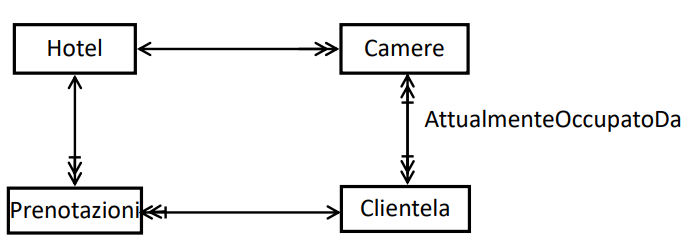
\includegraphics[scale=0.6]{img/esempioRelazione1.png}
\end{figure}

\subsubsection{Associazioni e Cardinalità}

Formalmente le associazioni sono insiemi di coppie, quindi delle relazioni. Il tipo di freccetta che indica l'associazione
è detta cardinalità e corrisponde informalmente alla domanda:

\[ \text{"Per ogni elemento della classe A quanti della classe B?"} \]

Chiaramente va fatto sulla stessa direzione per entrambi i versi. Questo permette di risolvere le ambiguità causate dalla terminologia comune che è detta:

\[ \text{"Uno a Molti"} \:\: \text{oppure} \:\: \text{"Molti a Molti"} \]

che in qualche modo genera ambiguità perchè è come se si tenesse in conto solo di un verso. E' fondamentale ricordarsi quindi che la caratterizzazione della cardinalità di un associazione va
fatta in entrambi i versi.

Graficamente quindi avremo queste possibilità alle estremità delle associazioni:

\begin{enumerate}
    \item \textbf{Freccia Singola}: Per ogni elemento della classe di partenza è presente un elemento nella classe d'arrivo.
    \item \textbf{Freccia Doppia}: Per ogni elemento della classe di partenza sono presenti più elementi nella classe d'arrivo.
    \item \textbf{Trattino}: Nessun limite inferiore, di conseguenza per ogni elemento della classe di partenza può anche non essere presente alcun elemento nella classe d'arrivo.
\end{enumerate}

Esistono diverse notazioni grafiche, ma queste dispense fanno riferimento a quelle utilizzate durante gli esercizi del corso, quindi questa sarà la notazione comune di riferimento.

\newpage

\subsubsection{Associazioni Ternarie/con Attributi e Reificazione}

A volte le associazioni potrebbero complicarsi perchè:

\begin{enumerate}
    \item Potrebbero avere la \textbf{necessità} di avere degli \textbf{attributi}. Ad esempio in un caso di associazione tra Clienti e Stanze, la tariffa potrebbe non essere
    nè attributo di Clienti e nè di Stanze. In questo caso si assegna un \textbf{attributo} all'\textbf{associazione}.

    \begin{figure}[htbp]
        \center
        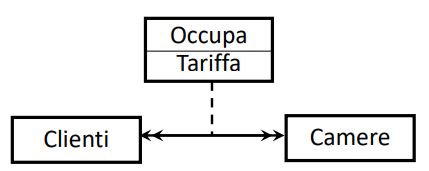
\includegraphics[scale=0.55]{img/associazioneAttributo.png}
    \end{figure}

    \item Potrei invece immaginare l'attributo come \textbf{vera} e \textbf{propria entità} di una specifica classe Tariffe. In quel caso non starei semplicemente dando 
    un attributo 

    
    all'associazione ma starei componendo un \textbf{associazione ternaria}.
    \begin{figure}[htbp]
        \center
        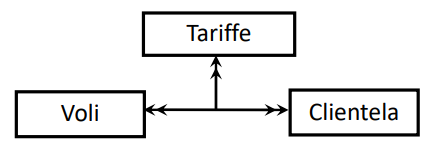
\includegraphics[scale=0.55]{img/associazioneTernaria.png}
    \end{figure}

\end{enumerate}

\paragraph{Reificazione} Si preferisce, nei casi illustrati sopra, semplificare la gestione 

dell'associazione tramite processo di reificazione, ossia la creazione di una classe di supporto aggiuntiva che permetta la gestione
regolare delle associazioni viste prima. Si illustrano le reificazioni delle associazioni viste sopra:

\vspace*{15px}

\begin{figure}[htbp]
    \centering
    \begin{minipage}{0.45\textwidth}
        \centering
        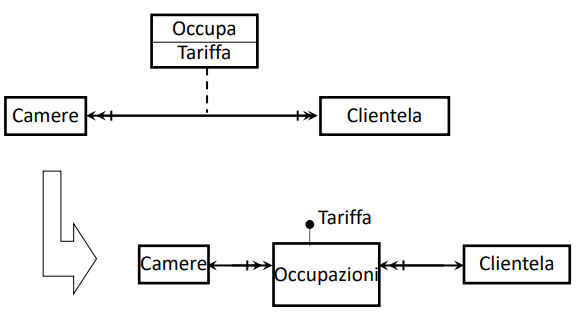
\includegraphics[width=\linewidth]{img/esempioReificazione1.png}
        \caption{Reificazione di Associazione con Attributo}
    \end{minipage}
    \hfill
    \begin{minipage}{0.45\textwidth}
        \centering
        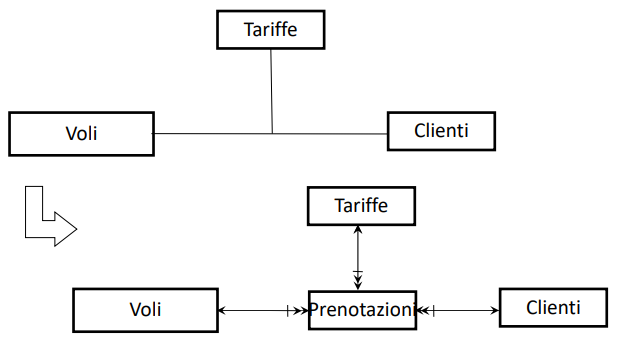
\includegraphics[width=\linewidth]{img/esempioReificazione2.png}
        \caption{Reificazione di Associazione Ternaria}
    \end{minipage}
\end{figure}

Un dettaglio da notare è la \textbf{cardinalità} sulla nuova classe di supporto, infatti in \textbf{direzione} della \textbf{nuova classe} sarà presente un associazione di \textbf{uno a molti}.

\newpage

\subsubsection{Sottoclassi e Tipologie}

Una \textbf{sottoclasse} è un sottoinsieme di elementi di una classe, per i quali prevediamo di raccogliere ulteriori informazioni.

\[ \text{Studenti} \subseteq \text{Persone} \]
\[ \text{Libri Rari} \subseteq \text{Libri} \]

\begin{figure}[htbp]
    \center
    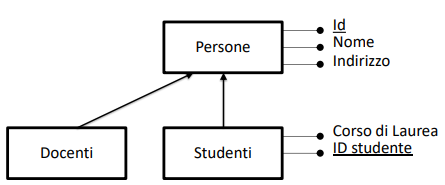
\includegraphics[scale=0.7]{img/notazioneGraficaSottoclassi.png}
    \caption{Notazione grafica di riferimento}
\end{figure}

\vspace*{10px}

Esistono varie tipologie di sottoclassi:

\vspace*{10px}

\begin{figure}[htbp]
    \center
    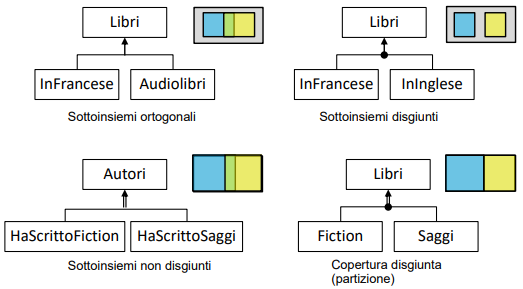
\includegraphics[scale=0.7]{img/tipiDiSottoclassi.png}
\end{figure}

\newpage

\subsection{Progettazione Logica}

Il \textbf{tipo} di \textbf{schema logico} presentato in questo corso è lo \textbf{schema relazionale}.

\vspace*{10px}

Basata su \textbf{schemi relazionali} detti informalmente \textbf{tabelle} di valori elementari con chiavi primarie:

\vspace*{5px}

\begin{center}
\begin{tabular}{ |c|c|c|c| }
    \hline
    \multicolumn{4}{|c|}{Impiegati} \\
    \hline
    \underline{IdImpiegato} & Nome & Stipendio & IdReparto* \\
    \hline
    232 & Lucia & 1200 & Y1 \\
    \hline
    143 & Luigi & 1500 & X2 \\
    \hline
\end{tabular}
\end{center}

\vspace*{5px}

In questo contesto \textbf{non esiste differenza} tra \textbf{attributi} ed \textbf{associazioni} dato che le chiavi
esterne permetteranno il \textbf{riferimento} ad \textbf{altre tabelle}.

\vspace*{5px}

\begin{center}
\begin{tabular}{ |c|c| }
    \hline
    \multicolumn{2}{|c|}{Reparti} \\
    \hline
    \underline{IdReparto} & Budget \\
    \hline
    Y1 & 100000 \\
    \hline
    X2 & 200000 \\
    \hline
\end{tabular}
\end{center}

\vspace*{5px}

Solitamente quindi si definisce \textbf{uno dei campi} della \textbf{tabella} come \textbf{chiave primaria}, ossia che \textbf{identifica} univocamente \textbf{la riga}. Invece il campo che permette la dereferenziazione univoca
di una riga in un altra tabella è detta \textbf{chiave esterna}, che corrisponde alla \textbf{chiave primaria} della \textbf{tabella esterna}.

\paragraph{Chiave e Superchiave Minimale} Definiamo \textbf{superchiave} qualsiasi \textbf{insieme di attributi} che \textbf{non} può \textbf{ripetersi} in \textbf{righe diverse}. Si definisce \textbf{chiave} una \textbf{superchiave minimale}, ossia un insieme di attributi a cui
non possiamo rimuovere alcun attributo. Sarà quindi scelta del progettista scegliere una \textbf{chiave primaria tra} tutte le \textbf{chiavi possibili}.

\subsection{Da Schema Concettuale a Schema Logico - Fasi}

Elenchiamo e descriviamo le fasi necessarie per il passaggio da schema \textbf{concettuale} a \textbf{logico}.

\begin{enumerate}
    \item Aggiungere una \textbf{chiave primaria} artificiale ad ogni collezione che ne ha bisogno.
    \begin{enumerate}
        \item Una chiave deve essere \textbf{immutabile}, \textbf{muta}, ossia non deve portare con se alcuna informazione, ed \textbf{invisibile} agli utenti.
    \end{enumerate}
    \item Tradurre le \textbf{associazioni} e le \textbf{inclusioni} in \textbf{chiavi esterne}.
    \begin{enumerate}
        \item Una associazione $1-N$ diventano \textbf{chiavi esterne}.
        \item Una associazione $M-N$ diventano \textbf{tabelle} con due chiavi esterne che puntano alle tabelle tra cui esiste l'associazione.
    \end{enumerate}
    \item Tradurre gli \textbf{attributi multivalore} in \textbf{tabelle}.
    \item \textbf{Appiattire} gli \textbf{attributi complessi}, ossia da struct a lista di parametri semplici.
\end{enumerate}

% Ti manca la parte su ATTRIBUTI MULTIVALORE e PARTIZIONE DI TABELLE, attendi le slide

\newpage

%\begin{figure}[htbp]
    %\center
    %\includegraphics[scale=0.4]{img/classiComplessita2.png}
%\end{figure}


\end{document}